\section{Two NLG Tasks}
\label{sec:domains}

We will now focus the discussion on two specific NLG problems:
sentence generation in the sense of \citet{KolSto07}, and the
generation of instructions in virtual environments
\citep{ByrKolStrCasDalMooObe09}. For each, we will introduce the task
and show by example how the task can be seen as a planning problem.


\subsection{Sentence generation as planning}
\label{sec:domain-crisp}

One way of modelling the sentence generation problem is to assume a
lexicalized grammar in which each lexicon entry specifies how it can
be combined grammatically with the other lexicon entries, what piece
of meaning it expresses, and what the pragmatic conditions on using it
are. Sentence generation can then be seen as constructing a
grammatical derivation that is syntactically complete, respects the
semantic and pragmatic conditions, and achieves all the
\emph{communicative goals}.

An example is the tree-adjoining grammar (TAG;
\citealt{joshi;etal1997}) shown in
Figure~\ref{fig:white-rabbit-sleeps-grammar}. This grammar consists of
\emph{elementary trees} (i.e., the disjoint trees in the figure), each
of which contributes certain \emph{semantic content}. Let's say that
we assume a knowledge base containing the individuals $e$, $r_1$ and
$r_2$ and the facts that $r_1$ and $r_2$ are rabbits, $r_1$ is white
and $r_2$ is brown, and $e$ is an event in which $r_1$ sleeps. Then we
would want to construct a sentence expressing the information
$\{\mathsf{sleep}(e,r_1)\}$ by combining instances of the elementary
trees (in which the \emph{semantic roles}, such as $\mathsf{self}$ and
$\mathsf{subj}$, have been substituted by constants from the knowledge
base) into a TAG derivation as as shown in
Figure~\ref{fig:white-rabbit-sleeps-deriv}. In the picture, the dashed
arrow indicates TAG's \emph{substitution} operation, which ``plugs''
an elementary into the leaf of another tree, and the dotted arrows
stand for \emph{adjunction}, which splices an elementary tree into an
internal node. We can then read off the sentence ``The white rabbit
sleeps'' from the derivation. Note that the sentence ``The rabbit
sleeps'' would not have been an appropriate result, because ``the
rabbit'' could refer to either $r_1$ or $r_2$, and thus $r_2$ remains
as a \emph{distractor}, i.e.\ an incorrect possible interpretation of
the phrase.

\begin{figure}
  \centering
  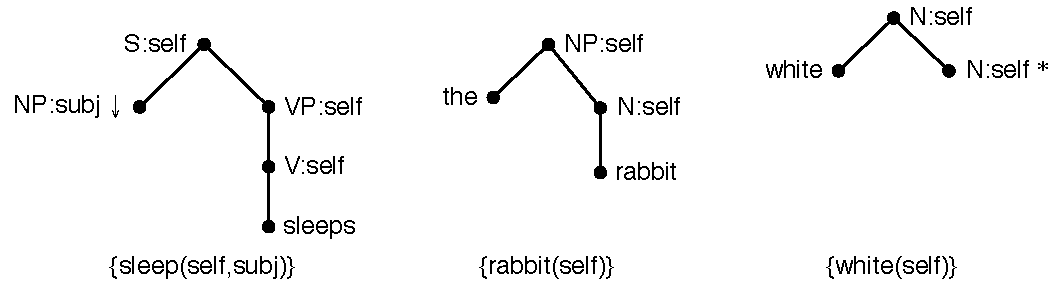
\includegraphics[width=0.75\columnwidth]{pic-grammar}
  \caption{An example grammar in the sentence generation domain.}
  \label{fig:white-rabbit-sleeps-grammar}
\end{figure}

\begin{figure}
  \centering
  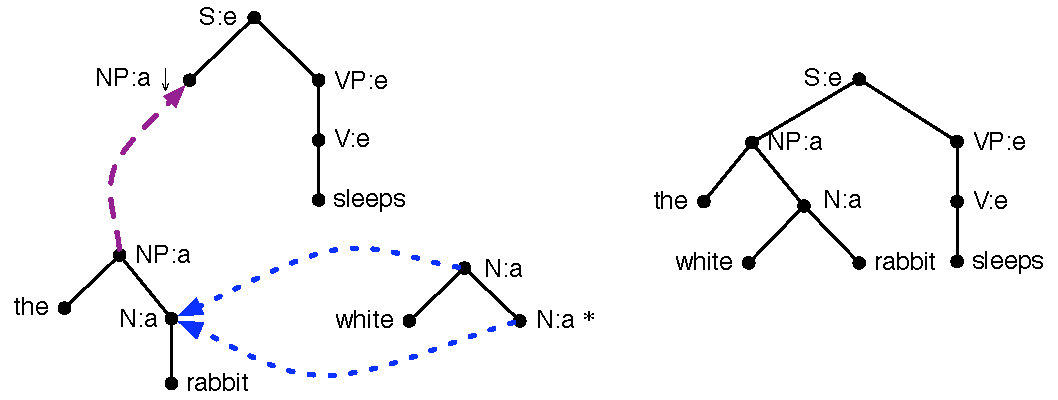
\includegraphics[width=0.75\columnwidth]{pic-derivation}
  \caption{Derivation of ``The white rabbit sleeps.''}
  \label{fig:white-rabbit-sleeps-deriv}
\end{figure}

This perspective on sentence generation has the advantage of solving
the sentence planning and surface realization problems
simultaneously. The generation of referring expressions (REs) is
usually seen as a sentence planning task; in the example, we required
that the referring expression ``the white rabbit'' can be resolved
uniquely to $r_1$ by the hearer, in addition to the requirement that
the derivation is grammatically correct. This is useful in cases where
sentence planning and surface realization interact, because syntactic
information about the individual words is available when the REs are
generated (see e.g. \citealt{stone98textual}). However, the problem of
whether a given communicative goal can be achieved with a given
grammar is NP-complete \citep{KolStr02}. A naive search algorithm that
computes the derivation top-down takes exponential time and is clearly
infeasible to use in practice. The seminal SPUD system
\citep{Stone2003a}, which first worked out the idea of integrated
TAG-based sentence generation, used a greedy algorithm to cope with
the search, which circumvents the combinatorial explosion but is
incomplete.

\begin{figure}
\centering
\begin{minipage}{0.8\textwidth}
{\small%
\begin{verbatim}
(:action add-sleeps
   :parameters (?u - node  ?xself - individual  ?xsubj - individual)
   :precondition
       (and (subst S ?u)  (referent ?u ?xself)  (sleep ?xself ?xsubj))
   :effect 
       (and (not (subst S ?u))  (expressed sleep ?xself ?xsubj)
            (subst NP (subj ?u))  (referent (subj ?u) ?xsubj)
            (forall (?y - individual)
                (when (not (= ?y ?xself)) (distractor (subj ?u) ?y)))))

(:action add-rabbit
   :parameters (?u - node  ?xself - individual)
   :precondition 
       (and (subst NP ?u)  (referent ?u ?xself)  (rabbit ?xself))
   :effect 
       (and (not (subst NP ?u))  (canadjoin N ?u)
            (forall (?y - individual)
                (when (not (rabbit ?y)) (not (distractor ?u ?y))))))

(:action add-white
   :parameters (?u - node  ?xself - individual)
   :precondition 
       (and (canadjoin N ?u)  (referent ?u ?xself)  (rabbit ?xself))
   :effect 
       (forall (?y - individual)
           (when (not (white ?y)) (not (distractor ?u ?y)))))
\end{verbatim}}%
\end{minipage}
\caption{PDDL actions for generating the sentence ``The white rabbit
sleeps.''}
\label{fig:white-rabbit-as-planning}
\end{figure}

As an alternative, \citet{KolSto07} recently proposed to control the
search by converting the sentence generation problem into a planning
problem and then running a planner \citet{KolSto07}.\footnote{See
  \url{http://code.google.com/p/crisp-nlg/} for the CRISP system, in
  which this conversion is implemented.} This planning problem assumes
an initial state containing an atom $\mathsf{subst}(S,\mathsf{root})$,
encoding that we must generate a sentence ($S$) starting at the node
named $\mathsf{root}$ in the TAG derivation tree, and an atom
$\mathsf{referent}(\mathsf{root},e)$ encoding that the (event)
individual which the entire sentence describes is $e$. Then it encodes
the addition of elementary trees to the TAG derivation in the
individual planning operators; the ones that are needed for our
example above are shown in
Fig.~\ref{fig:white-rabbit-as-planning}.

Here the action instance $\addact{sleeps}(\mathsf{root}, e, r_1)$
replaces the atom $\mathsf{subst}(S,\mathsf{root})$ with the atom
$\mathsf{subst}(NP,\mathsf{subj}(\mathsf{root}))$. In an abuse of PDDL
syntax, we write $\mathsf{subj}(\mathsf{root})$ as shorthand for a
fresh individual name.\footnote{These terms, which are not valid in
  ordinary PDDL, can be eliminated by estimating an upper bound $n$
  for the plan length, making $n$ copies of each action, ensuring that
  copy $i$ can only be applied in step $i$, and replacing the term
  $\mathsf{subj}(u)$ in an action copy by the constant
  $\mathsf{subj}_i$. The terms $S$, $NP$, and $N$ in the planning
  problem are constants.}  At the same time, the operator records that
the semantic information $\mathsf{sleep}(e,r_1)$ has now been
expressed, and introduces all individuals except for $r_1$ as
distractors for the new RE at $\mathsf{subj}(\mathsf{root})$. These
distractors can then be removed by subsequent applications of the
other two operators. Eventually we reach a goal state, which is
characterized by goals including $\forall x \forall y. \neg
\mathsf{subst}(x,y)$, $\forall x \forall y. \neg
\mathsf{distractor}(x,y)$, and
$\mathsf{expressed}(\mathsf{sleep},e,r_1)$. In summary, the following
is a correct plan:
%
\begin{enumerate}
\item $\mathsf{add}\textsf{-}\mathsf{sleeps}(\mathsf{root}, r_1)$,
\item $\mathsf{add}\textsf{-}\mathsf{rabbit}(\mathsf{subj}(\mathsf{root}),r_1)$,
\item $\mathsf{add}\textsf{-}\mathsf{white}(\mathsf{subj}(\mathsf{root}),r_1)$.
\end{enumerate}
%
The grammatical derivation in
Figure~\ref{fig:white-rabbit-sleeps-deriv}, and therefore the
generated sentence ``the white rabbit sleeps'', can be systematically
reconstructed from this plan. Thus, we can solve the sentence
generation problem via the detour through planning and bring current
search heuristics for planning to bear on generation.


\subsection{Planning in instruction giving}
\label{sec:domain-give}

Let us now turn to a second recent application of planning in NLG, the
GIVE Challenge (``Generating Instructions in Virtual Environments'';
\citealt{ByrKolStrCasDalMooObe09}). The object of this shared task is
to build an NLG system which produces natural-language instructions
which will guide a human user in performing some task in a virtual
environment.  From an NLG perspective, GIVE makes for an interesting
challenge because it is a theory-neutral task that exercises all
components of an NLG system, and emphasizes the study of communication
in a (simulated) physical environment. Furthermore, because the client
which displays the 3D environment to the user and the NLG system can
be physically separated, as long as they are connected over a network,
such systems can be cheaply evaluated over the Internet. This provides
a potential solution to the long-standing problem of evaluating NLG
systems. The first installment of GIVE (GIVE-1) evaluated five NLG
systems on the performance of 1143 users, making it the largest NLG
evaluation effort in terms of human users ever.

\begin{figure}[t]
\centering
%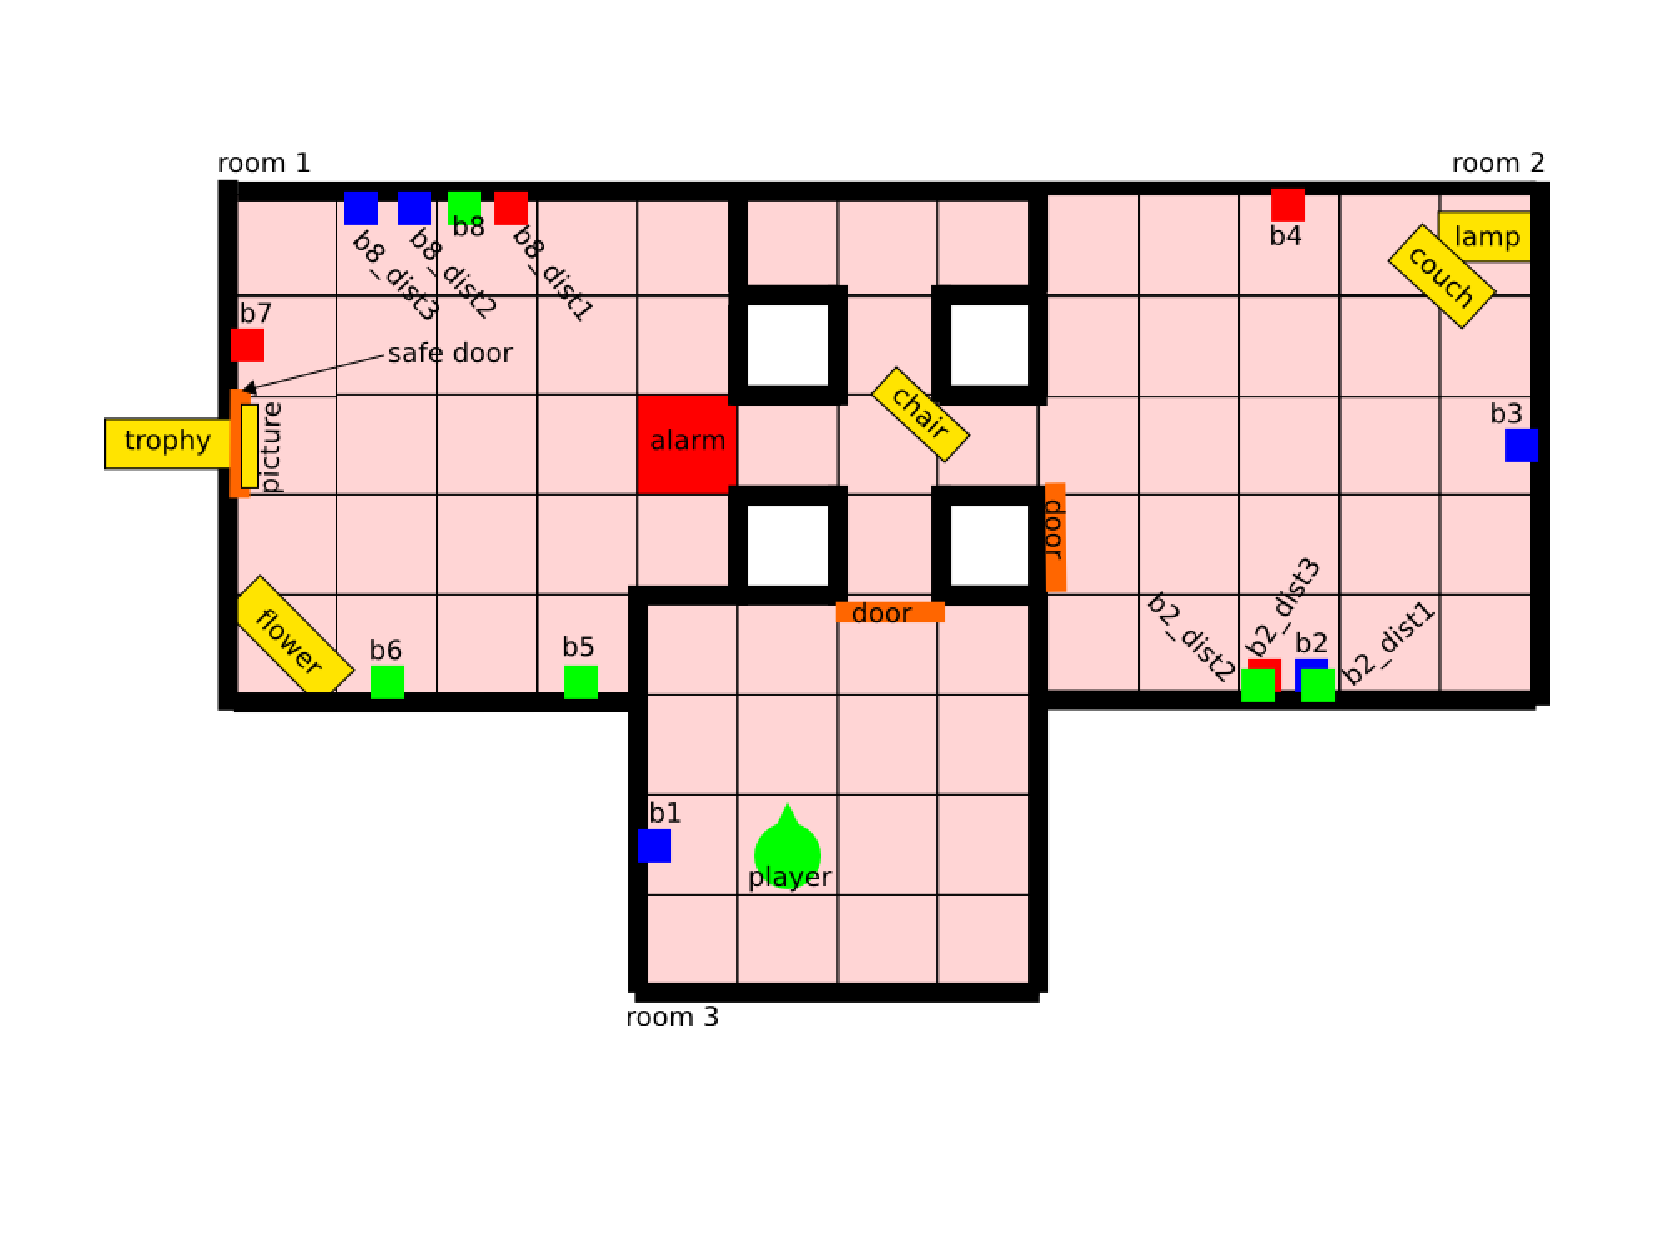
\includegraphics[width=1 \columnwidth]{give_world_no_expl}
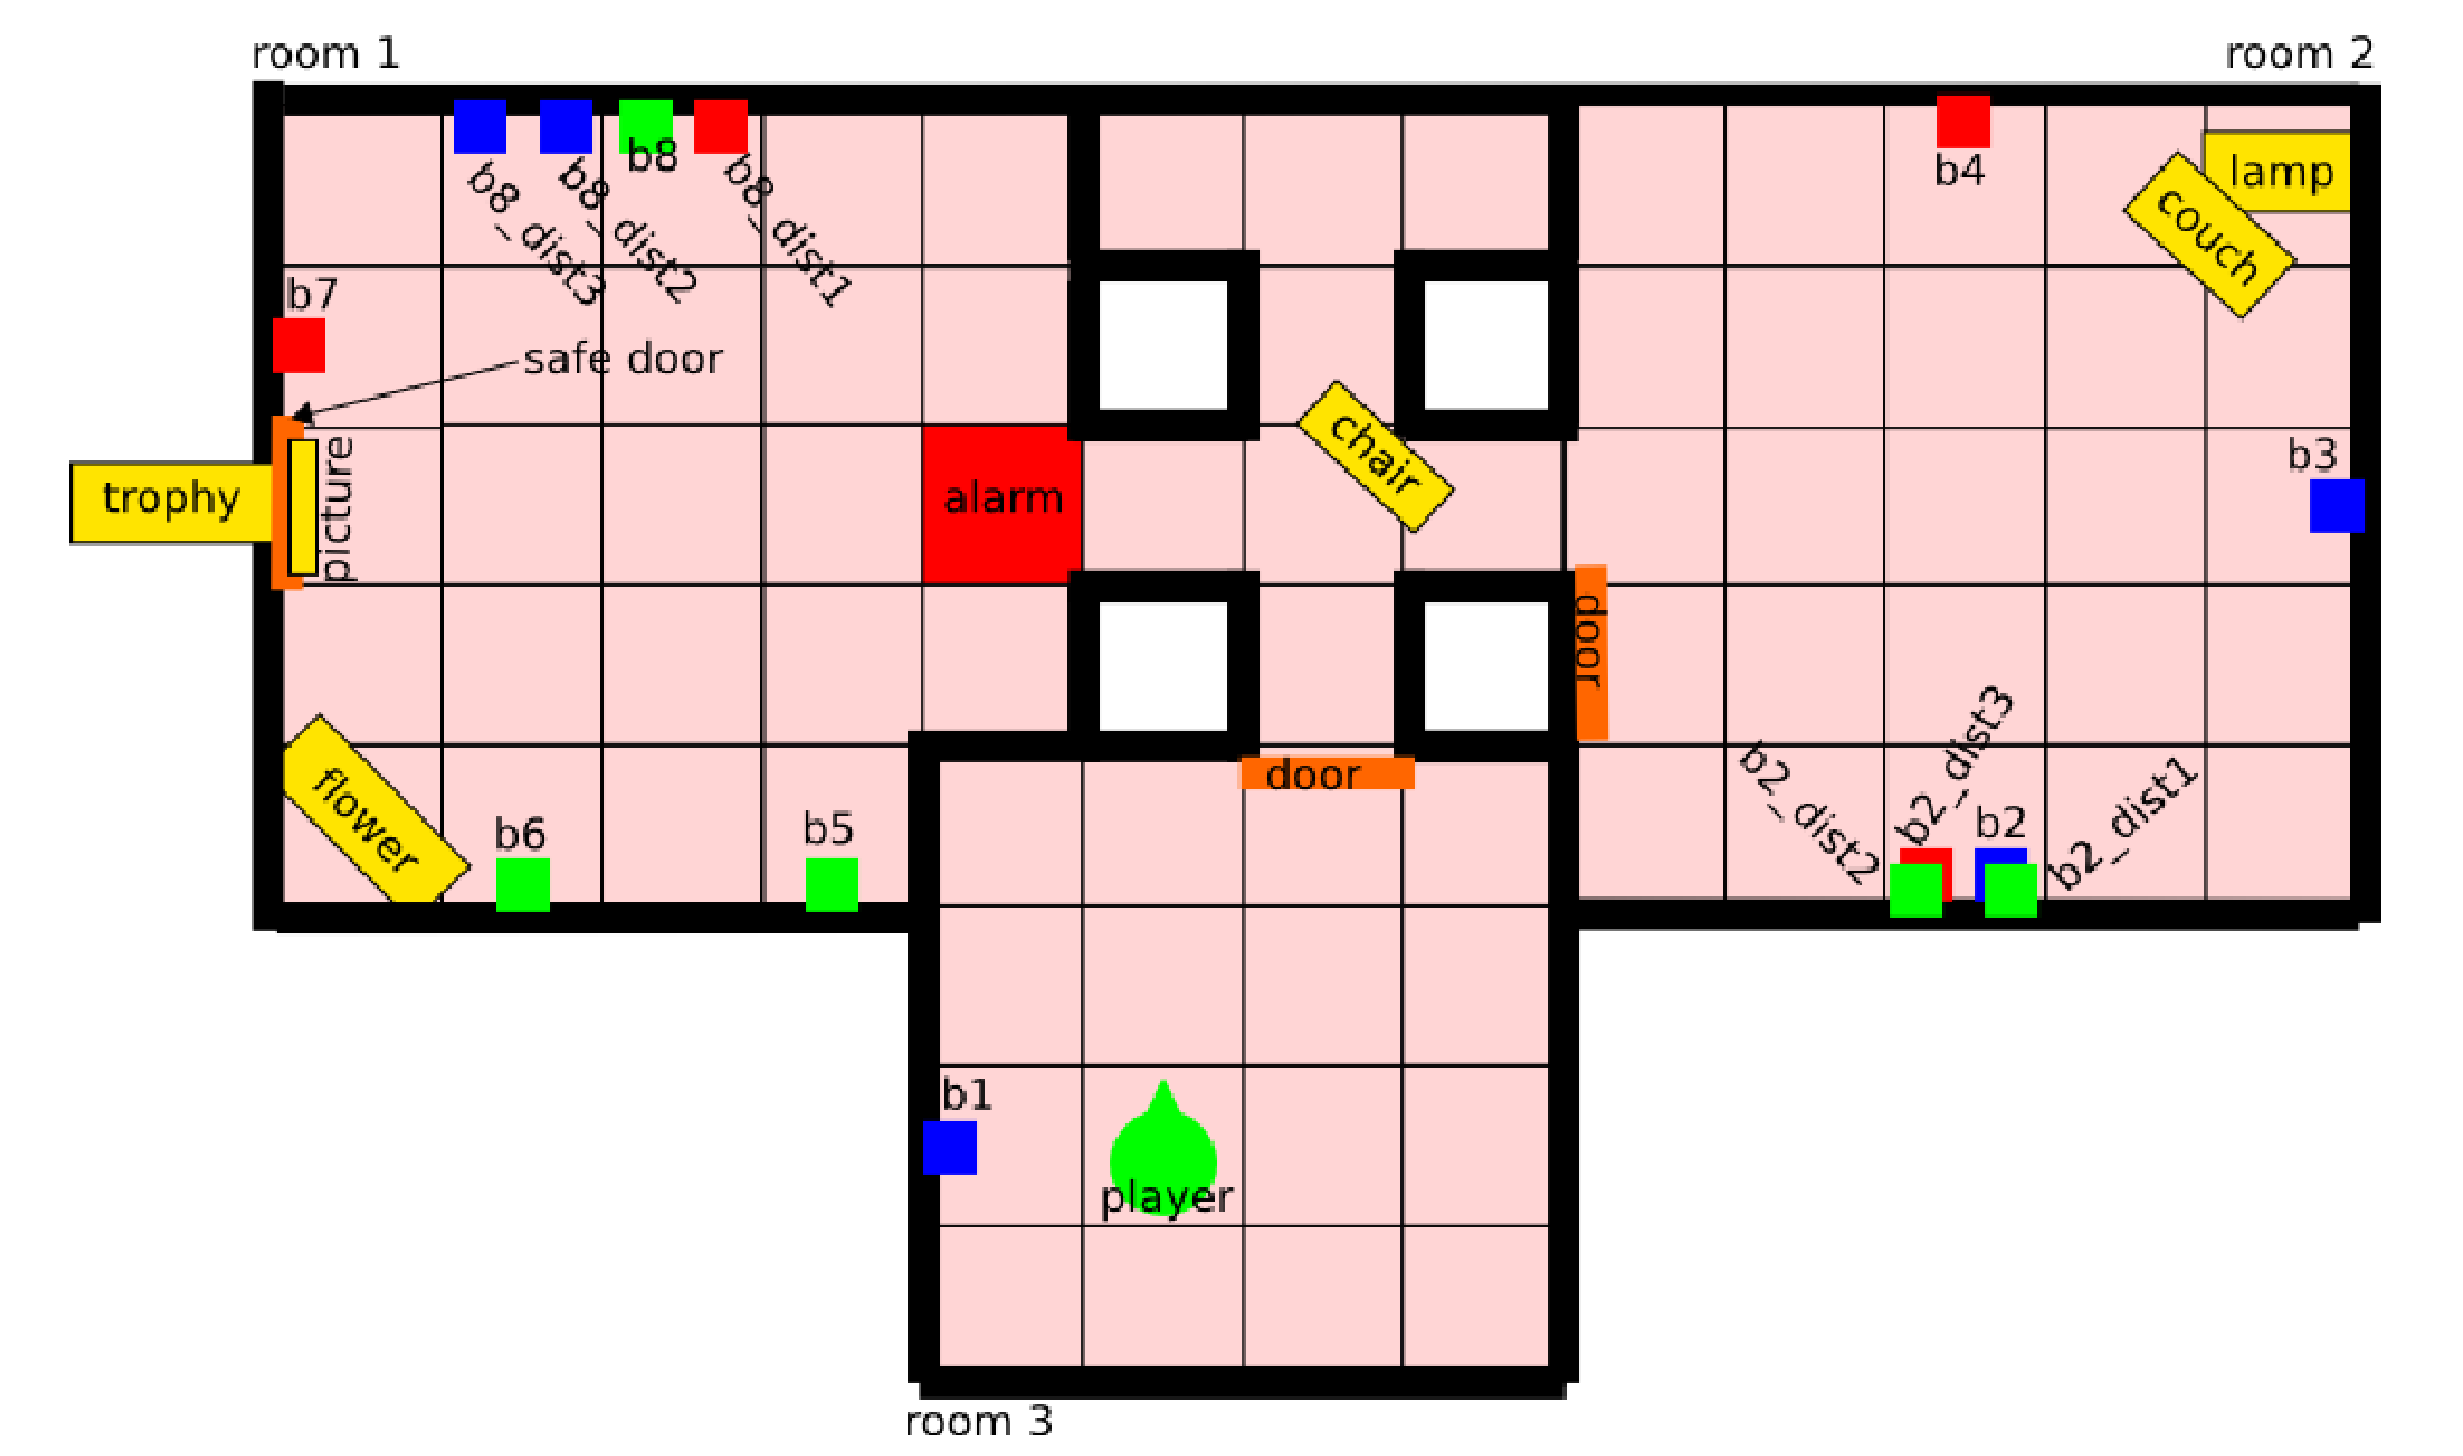
\includegraphics[width=0.75\columnwidth]{give_world_2}
\caption{Map of a GIVE world.}
  \label{fig:give-development-world}
\end{figure}

Planning plays a central role in the GIVE task. To see this, consider
the example GIVE world map in
Figure~\ref{fig:give-development-world}. In this example world, the
user's task is to pick up a trophy in the top left room. The trophy is
hidden in a safe behind a picture; to access it, the user must push
certain buttons in order to move the picture out of the way, open the
safe, and open doors. The user must to navigate the world and perform
these actions in the 3D client in a certain order; the NLG system must
instruct the user on how to do this.  To simplify both the planning
and the NLG task, the world is discretised into a set of tiles of
equal size. The user can turn by 90 degree steps in either direction,
and can move from the centre of one tile to the centre of the next
tile, provided the path between two tiles is not blocked.
Figure~\ref{fig:give-planning} shows the encoding of some of the
available GIVE domain actions, in PDDL syntax. In the example, the
shortest plan to solve the task consists of 108 action steps, with the
first few steps as follows:
%
\begin{enumerate}
\item $\mathsf{turn}\textsf{-}\mathsf{left}(\mathsf{north},
\mathsf{west})$,
\item $\mathsf{move}(\mathsf{pos\_5\_2}, \mathsf{pos\_4\_2}, \mathsf{west})$,
\item $\mathsf{manipulate}\textsf{-}\mathsf{b1}\textsf{-}\mathsf{off}\textsf{-}\mathsf{on}(\mathsf{pos\_5\_2})$,
\item $\mathsf{turn}\textsf{-}\mathsf{right}(\mathsf{west}, \mathsf{north})$.
\end{enumerate}

\begin{figure}
\centering
\begin{minipage}{0.5\textwidth}
{\small%
\begin{verbatim}
(:action move
   :parameters (?from - position
                ?to - position
                ?ori - orientation)
   :precondition 
       (and (player-pos ?from) 
            (adjacent ?from ?to ?ori) 
            (player-orient ?ori)
            (not-blocked ?from ?to)
            (not-alarmed ?to))
   :effect 
       (and (not (player-pos ?from))
            (player-pos ?to)))

(:action turn-left
   :parameters (?ori - orientation
                ?newOri - orientation)
   :precondition 
       (and (player-orient ?ori)
            (next-orient-left ?ori ?newOri))
   :effect 
       (and (not (player-orient ?ori))
            (player-orient ?newOri)))

(:action turn-right
   :parameters (?ori - orientation
                ?newOri - orientation)
   :precondition 
       (and (player-orient ?ori)
            (next-orient-right ?ori ?newOri))
   :effect 
       (and (not (player-orient ?ori))
            (player-orient ?newOri)))

(:action manipulate-b1-off-on
   :parameters (?pos - position)
   :precondition 
       (and (state b1 off)
            (player-pos ?pos)
            (position b1 ?pos))
   :effect 
       (and (not (state b1 off))
            (state b1 on)
            (not (state d1 closed))
            (state d1 open) 
            (not (blocked pos_6_5 pos_6_4))
            (not (blocked pos_6_4 pos_6_5))))
\end{verbatim}}%
\end{minipage}
\caption{Some PDDL actions for the GIVE domain.}
\label{fig:give-planning}
\end{figure}

A GIVE NLG system must be able to compute such plans. At a minimum,
the discourse planner will call a planner in order to determine the
content of the instructions that should be presented to the
user. Under this view, the planning problem is very similar to the
Gridworld problem (see, e.g., \citealt{Tovey-Koenig:2000}), which also
involves finding a route through a two-dimensional world map with
discrete positions. As in Gridworld, the domain requires not only
route finding in the discretised world, but also the execution of
certain actions (such as finding keys and unlocking doors in
Gridworld, or pushing the correct buttons to open doors and the safe
in GIVE). However, the GIVE worlds tend to be bigger than the
Gridworld instances that were used in the 1990s planning competitions.

This relatively loose integration of NLG system and planner is the
state of the art of the systems that participated in GIVE-1. However,
it is desirable to integrate the planner and the generation system
more closely than this. For instance, let's say that the NLG system
wants to generate the instruction sequence ``walk to the centre of the
room; turn right; now press the green button in front of
you''. Experiments with human instruction givers \cite{stoia:08} show
that this is a pattern that they use frequently: The instruction
follower is made to walk to a certain point in the world at which the
instruction giver can then use a a referring expression (``the green
button'') that is very easy to interpret. Such an NLG system must
integrate discourse planning and planning in the domain of the world
map closely. On the one hand, the structure of the discourse is
determined by the needs of the NLG system rather than the domain plan;
on the other hand, the discourse planner must be aware of the way in
which the instruction ``turn right'' is likely to change the
visibility of objects. Even if the NLG system doesn't implement the
generation of this discourse as planning, it still solves a problem
that subsumes the domain planning problem. For these reasons, we
consider the GIVE domain planning problem as a natural part of a GIVE
NLG system.  \todo{Make sure that this paragraph still talks about the
  things that the reviewers found interesting about it.}

%%% Local Variables: 
%%% mode: latex
%%% TeX-master: "manuscript"
%%% End: 
